\documentclass[11pt]{article}

% Change "review" to "final" to generate the final (sometimes called camera-ready) version.
% Change to "preprint" to generate a non-anonymous version with page numbers.
\usepackage[review]{acl}

% Standard package includes
\usepackage{times}
\usepackage{latexsym}

% For proper rendering and hyphenation of words containing Latin characters (including in bib files)
\usepackage[T1]{fontenc}
% For Vietnamese characters
% \usepackage[T5]{fontenc}
% See https://www.latex-project.org/help/documentation/encguide.pdf for other character sets

% This assumes your files are encoded as UTF8
\usepackage[utf8]{inputenc}

% This is not strictly necessary, and may be commented out,
% but it will improve the layout of the manuscript,
% and will typically save some space.
\usepackage{microtype}

% This is also not strictly necessary, and may be commented out.
% However, it will improve the aesthetics of text in
% the typewriter font.
\usepackage{inconsolata}

%Including images in your LaTeX document requires adding
%additional package(s)
\usepackage{graphicx}

\usepackage{amsmath}
\usepackage{float}
\usepackage{subcaption}

\usepackage{orcidlink}
\usepackage{booktabs}

\usepackage{algorithm}
\usepackage{algpseudocode}
\usepackage{tabularx}

% If the title and author information does not fit in the area allocated, uncomment the following
%
%\setlength\titlebox{<dim>}
%
% and set <dim> to something 5cm or larger.

\title{Recursive Offline Distillation via Epistemic Complexity Approximation}

% Author information can be set in various styles:
% For several authors from the same institution:
% \author{Author 1 \and ... \and Author n \\
%         Address line \\ ... \\ Address line}
% if the names do not fit well on one line use
%         Author 1 \\ {\bf Author 2} \\ ... \\ {\bf Author n} \\
% For authors from different institutions:
% \author{Author 1 \\ Address line \\  ... \\ Address line
%         \And  ... \And
%         Author n \\ Address line \\ ... \\ Address line}
% To start a separate ``row'' of authors use \AND, as in
% \author{Author 1 \\ Address line \\  ... \\ Address line
%         \AND
%         Author 2 \\ Address line \\ ... \\ Address line \And
%         Author 3 \\ Address line \\ ... \\ Address line}

\author{
  \textbf{Andrey Goncharov\textsuperscript{1}},
  \textbf{Daniil Vyazhev\textsuperscript{1,2}},
  \textbf{Simon Epanov\textsuperscript{1}},
  \textbf{Alexey Zaytsev\textsuperscript{1}},
  \\
  \\
  \textsuperscript{1}Applied AI Institute,
  \\
  \small{
    \textbf{Correspondence:} \href{mailto:andrey@faillearnrepeat.net}{andrey@faillearnrepeat.net}
  }
}

\begin{document}
\maketitle
\begin{abstract}
  Distillation of reasoning chains from Large Language Models (LLMs) into their smaller siblings is a standard training approach.
  Quite frequently researchers do not have full access to a teacher model and its internal representations, which limits the resulting performance.
  We propose a novel blueprint for efficient offline distillation that recursively uses lightweight epistemic and aleatoric complexity approximations for selective distillation.
  Specifically, for three open models (3-4B) at each epoch we estimate offline data complexity with a single-token answer entropy and use a medium model's (70B) entropy as an aleatoric proxy.
  Next, we apply selective distillation only for a small subset of the reasoning chains with the highest corresponding epistemic component.
  Our approach consistently outperforms naive distillation on comparable computational budget ($57.15 \pm 1.01$ vs 51.61 on average) and offers a much steeper learning curve (baseline final score on ~15\% of the data).
  Additionally, we present comparative analysis of methods to generate, standardize and augment synthetic reasoning chains when the teacher model does not perform perfectly on the target distillation domain in the first place.
  We publish our code and data to facilitate further research in this direction.
\end{abstract}

\section{Introduction}

\begin{figure}
  \centering
  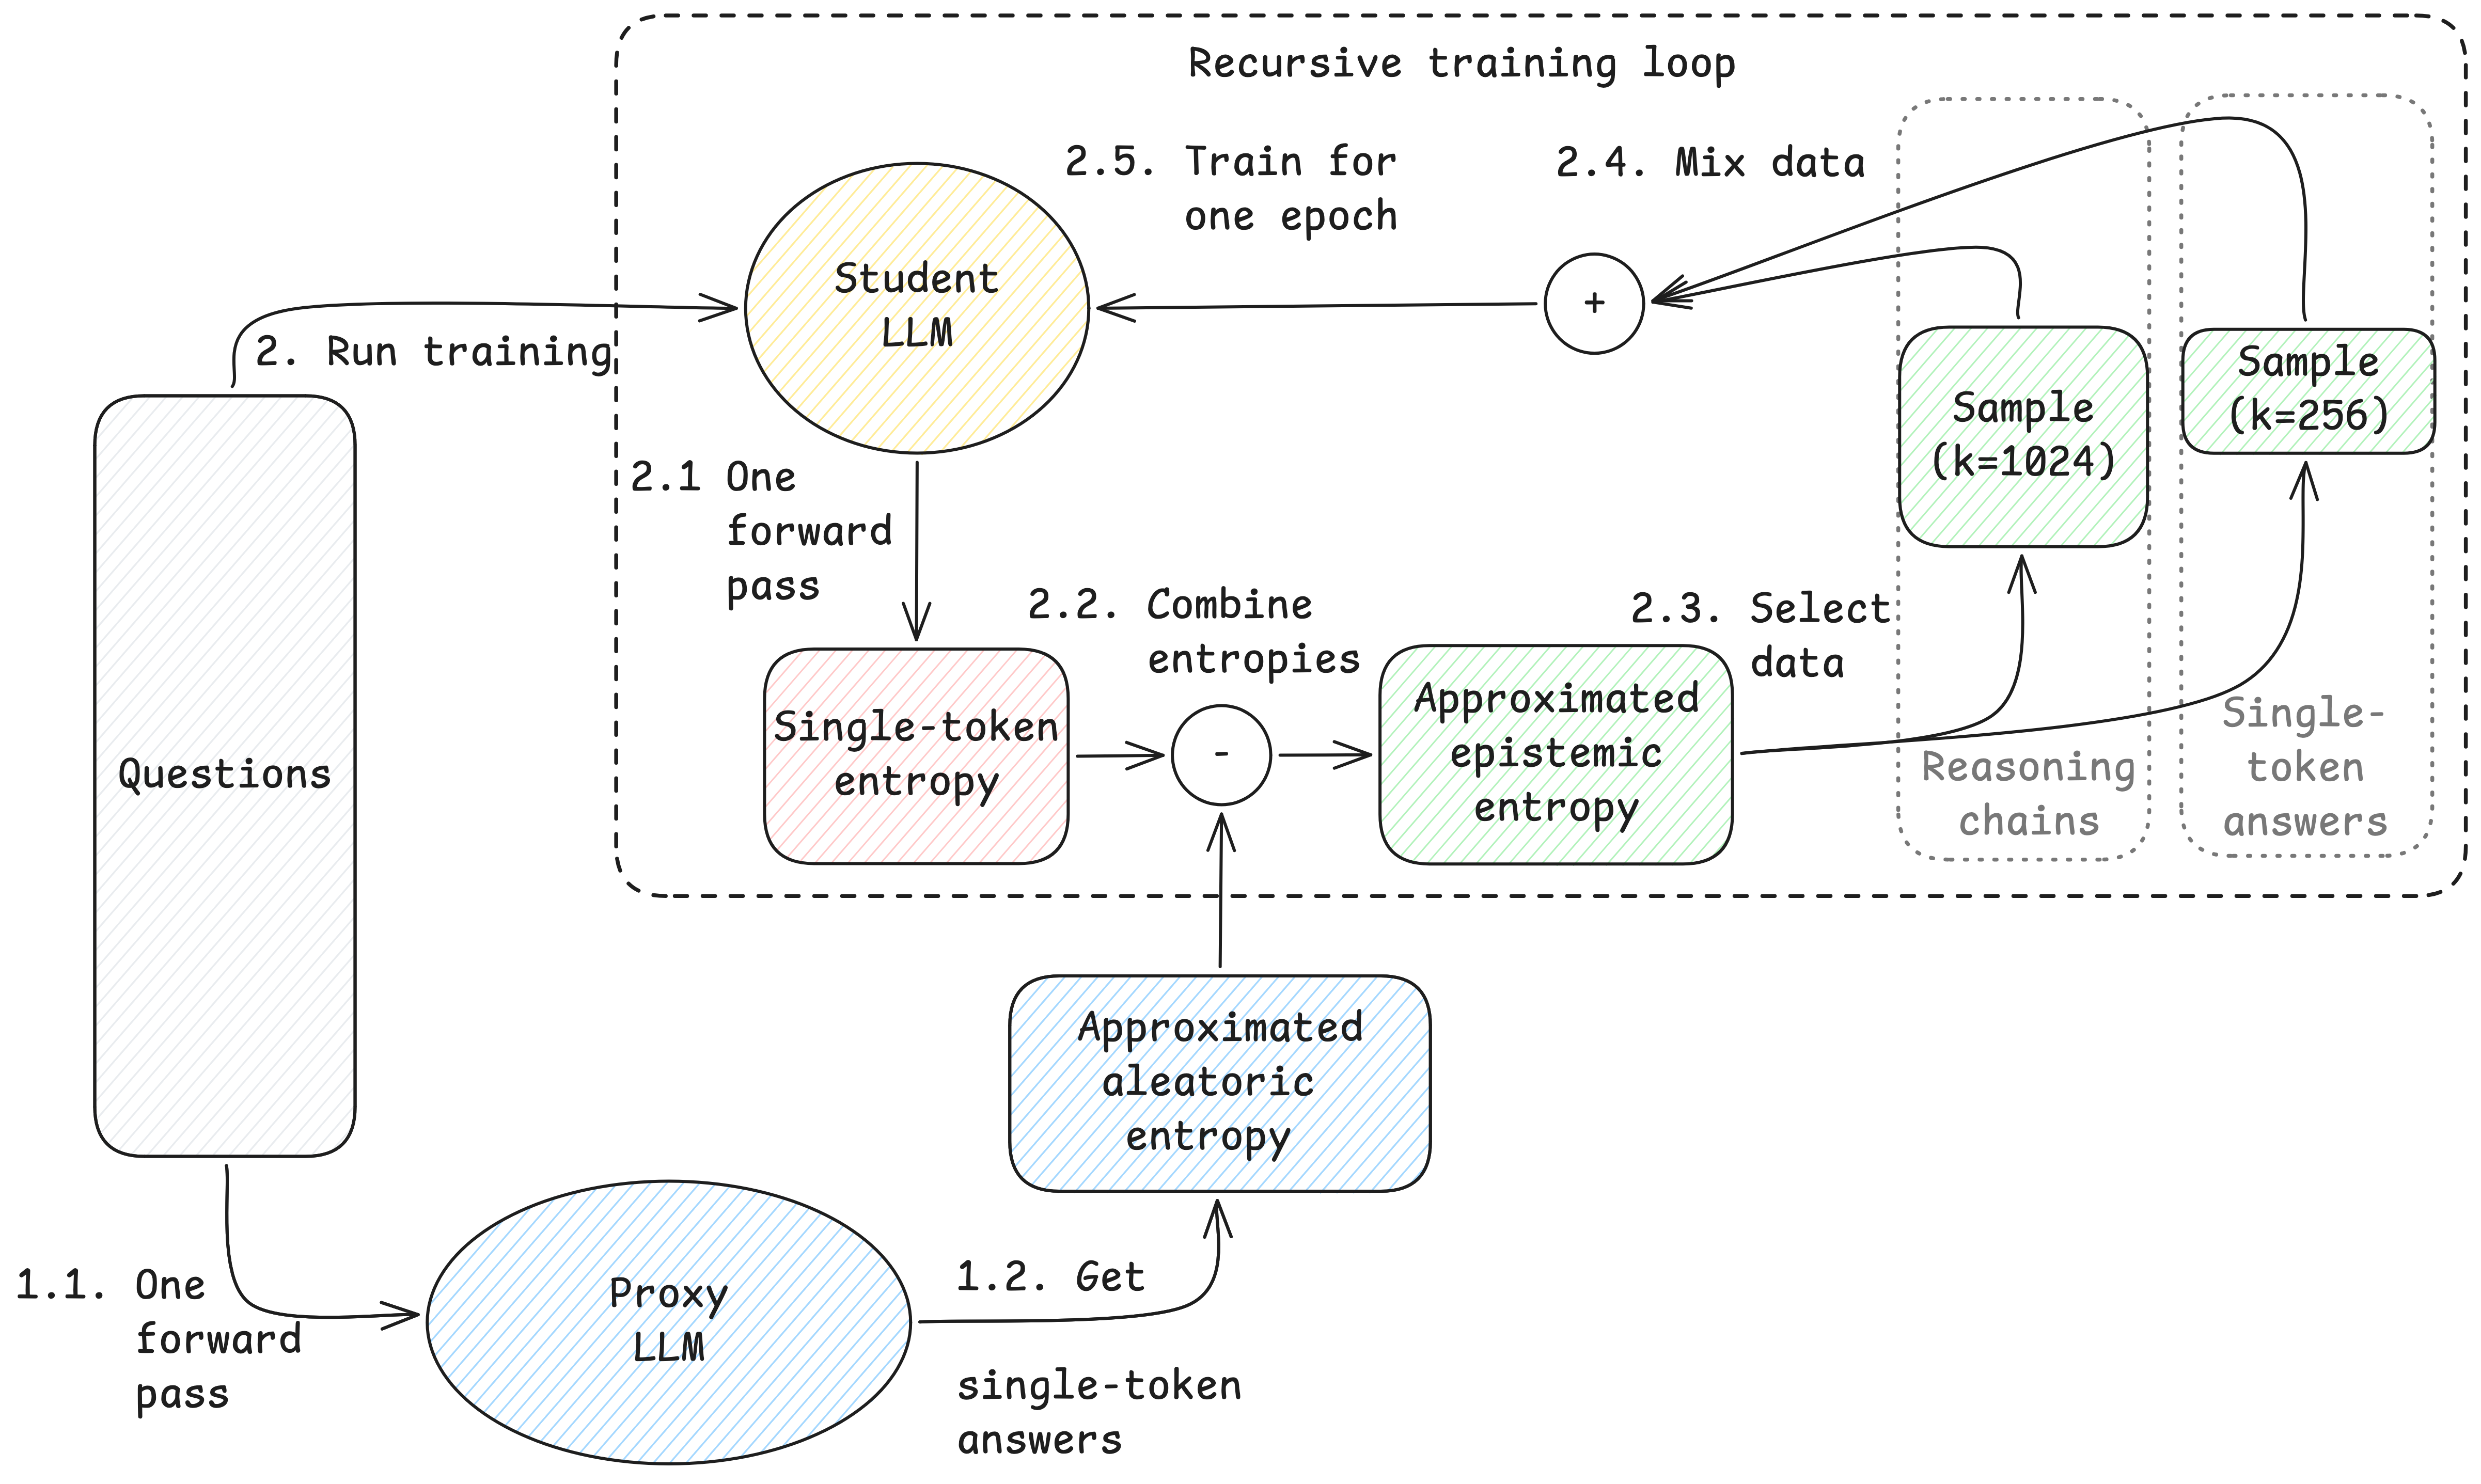
\includegraphics[width=1\linewidth]{img/recursive_caft_scheme.png}
  \caption{Recursive offline distillation scheme}
  \label{fig:recursive_caft_scheme}
\end{figure}

\section{Related Work}

\section{Methods}

\section{Results}

\subsection{Experimental Setup}

\subsection{Main Results}

\begin{figure*}
  \centering
  \begin{subfigure}[b]{0.48\linewidth}
    \centering
    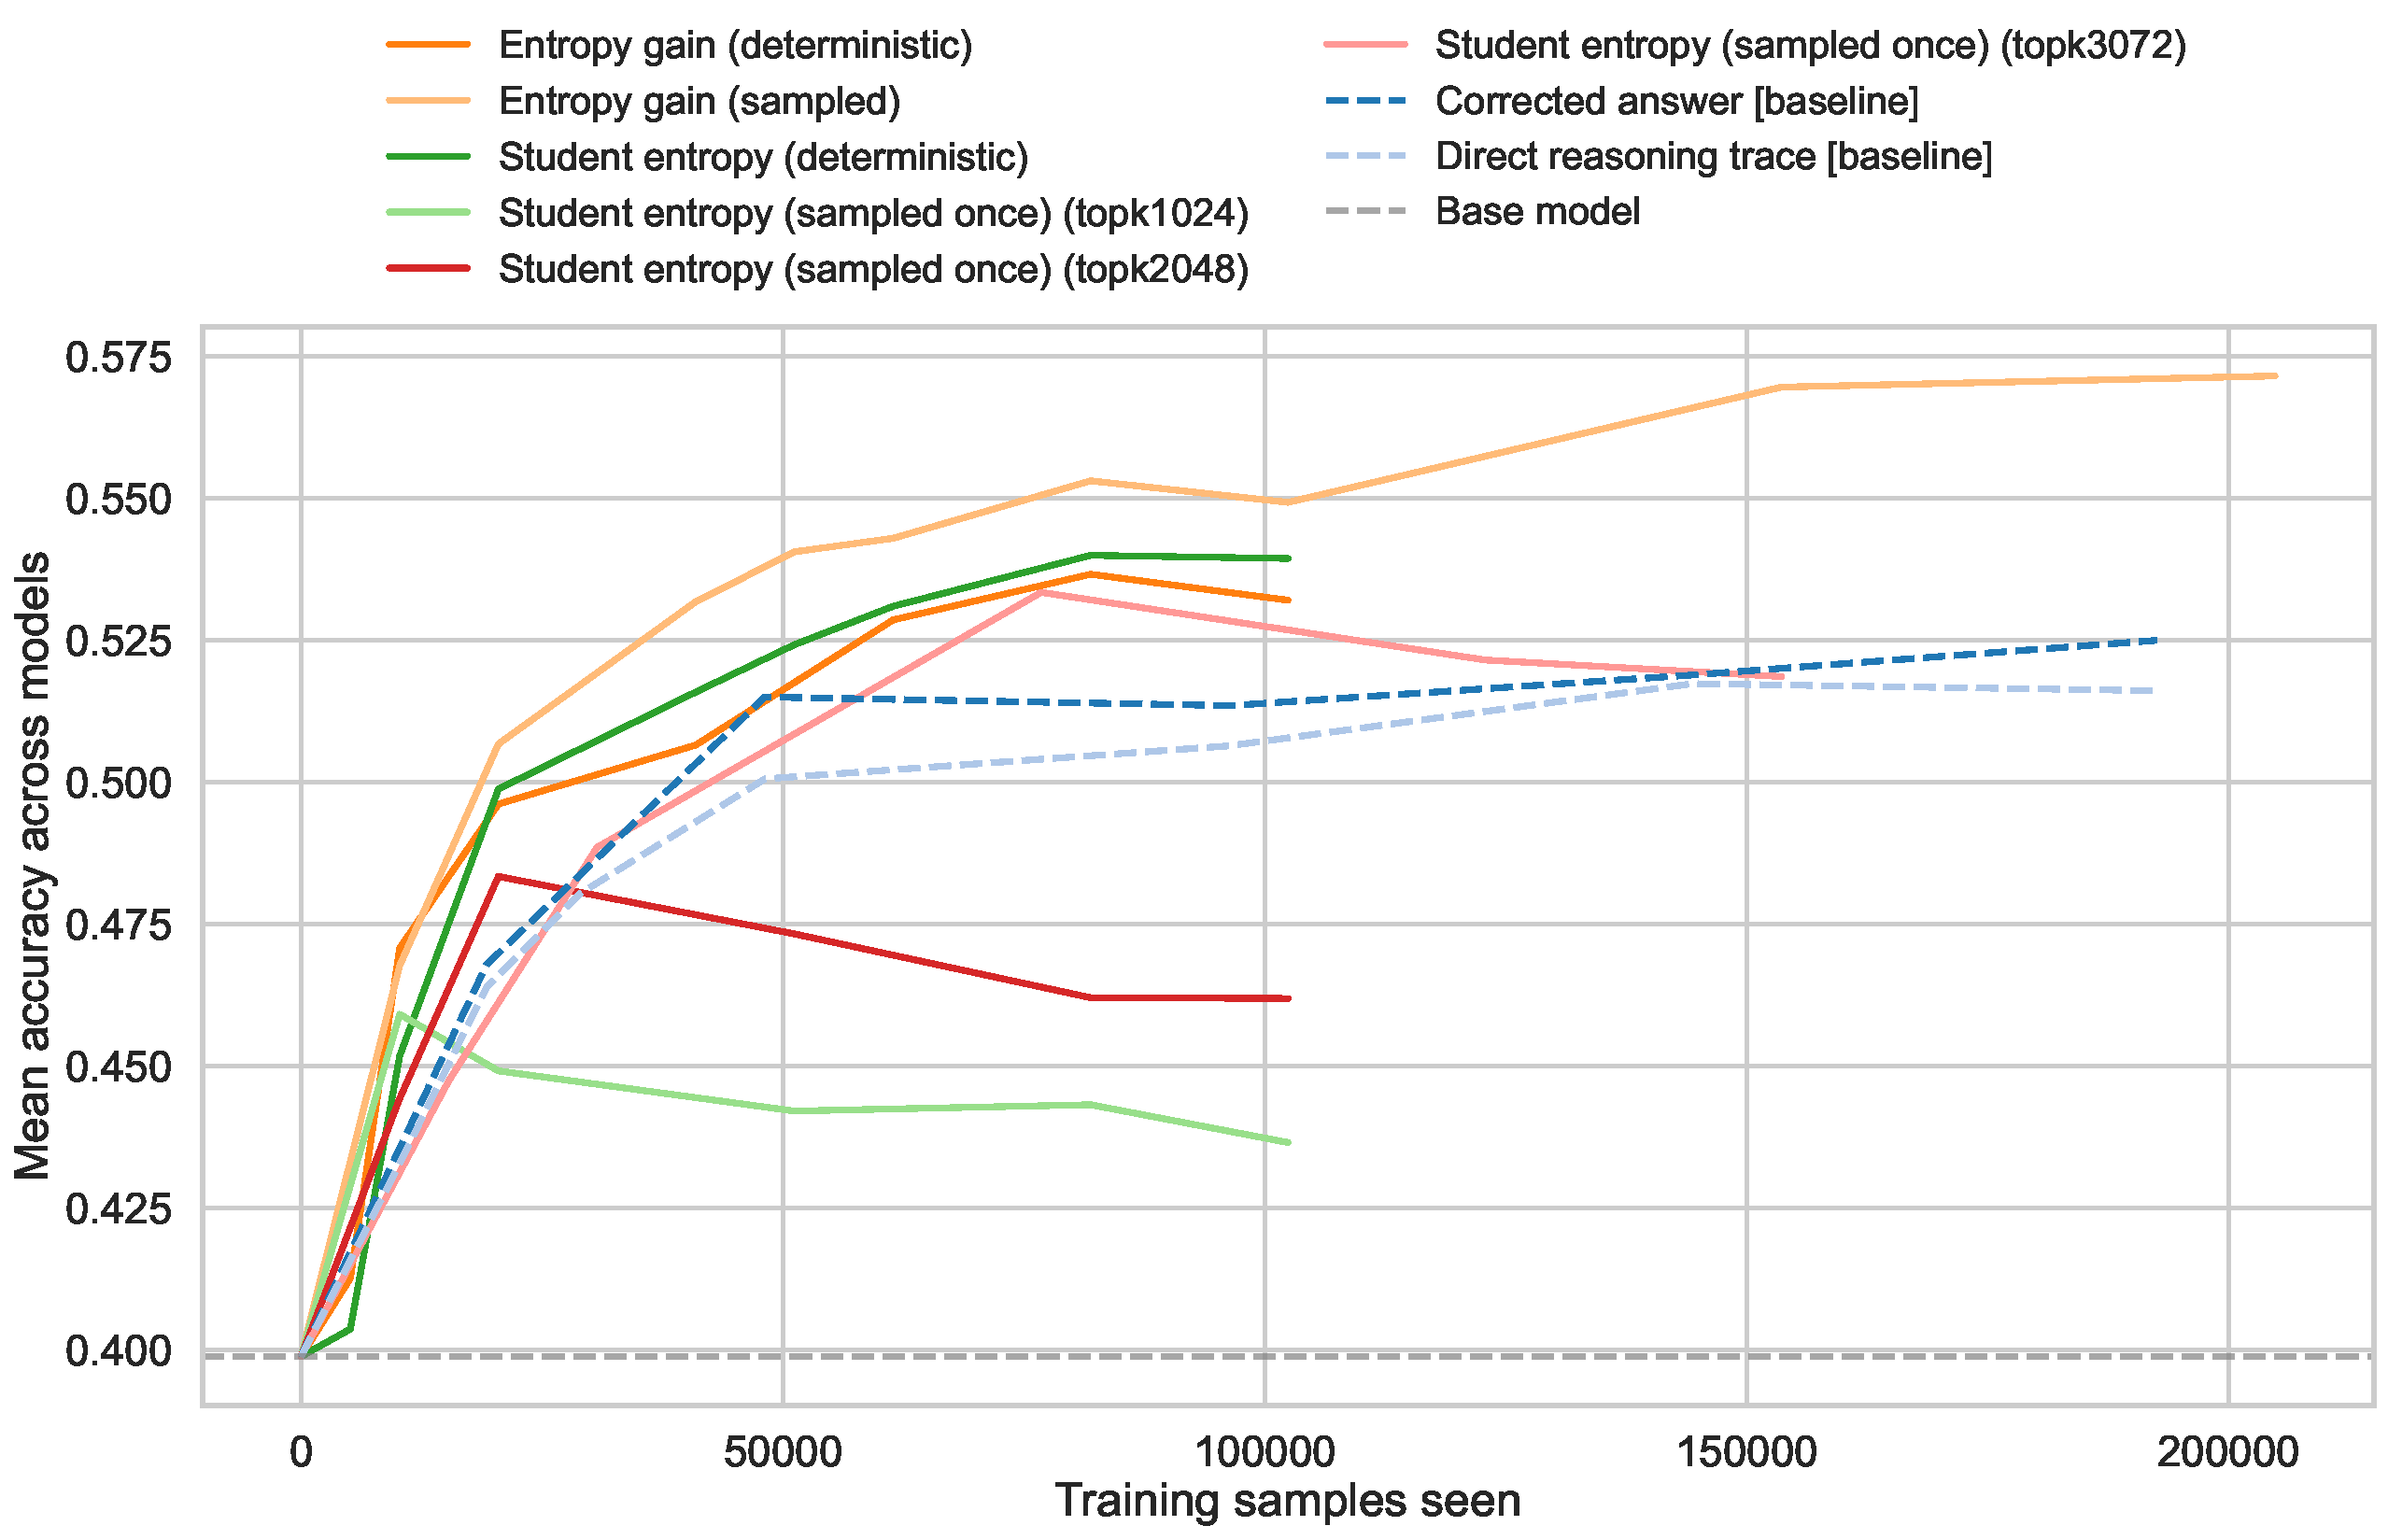
\includegraphics[width=1\linewidth]{img/all_models_reasoning_evals_cap4096.pdf}
    \caption{4096-token reasoning cap}
  \end{subfigure}
  \hfill
  \begin{subfigure}[b]{0.48\linewidth}
    \centering
    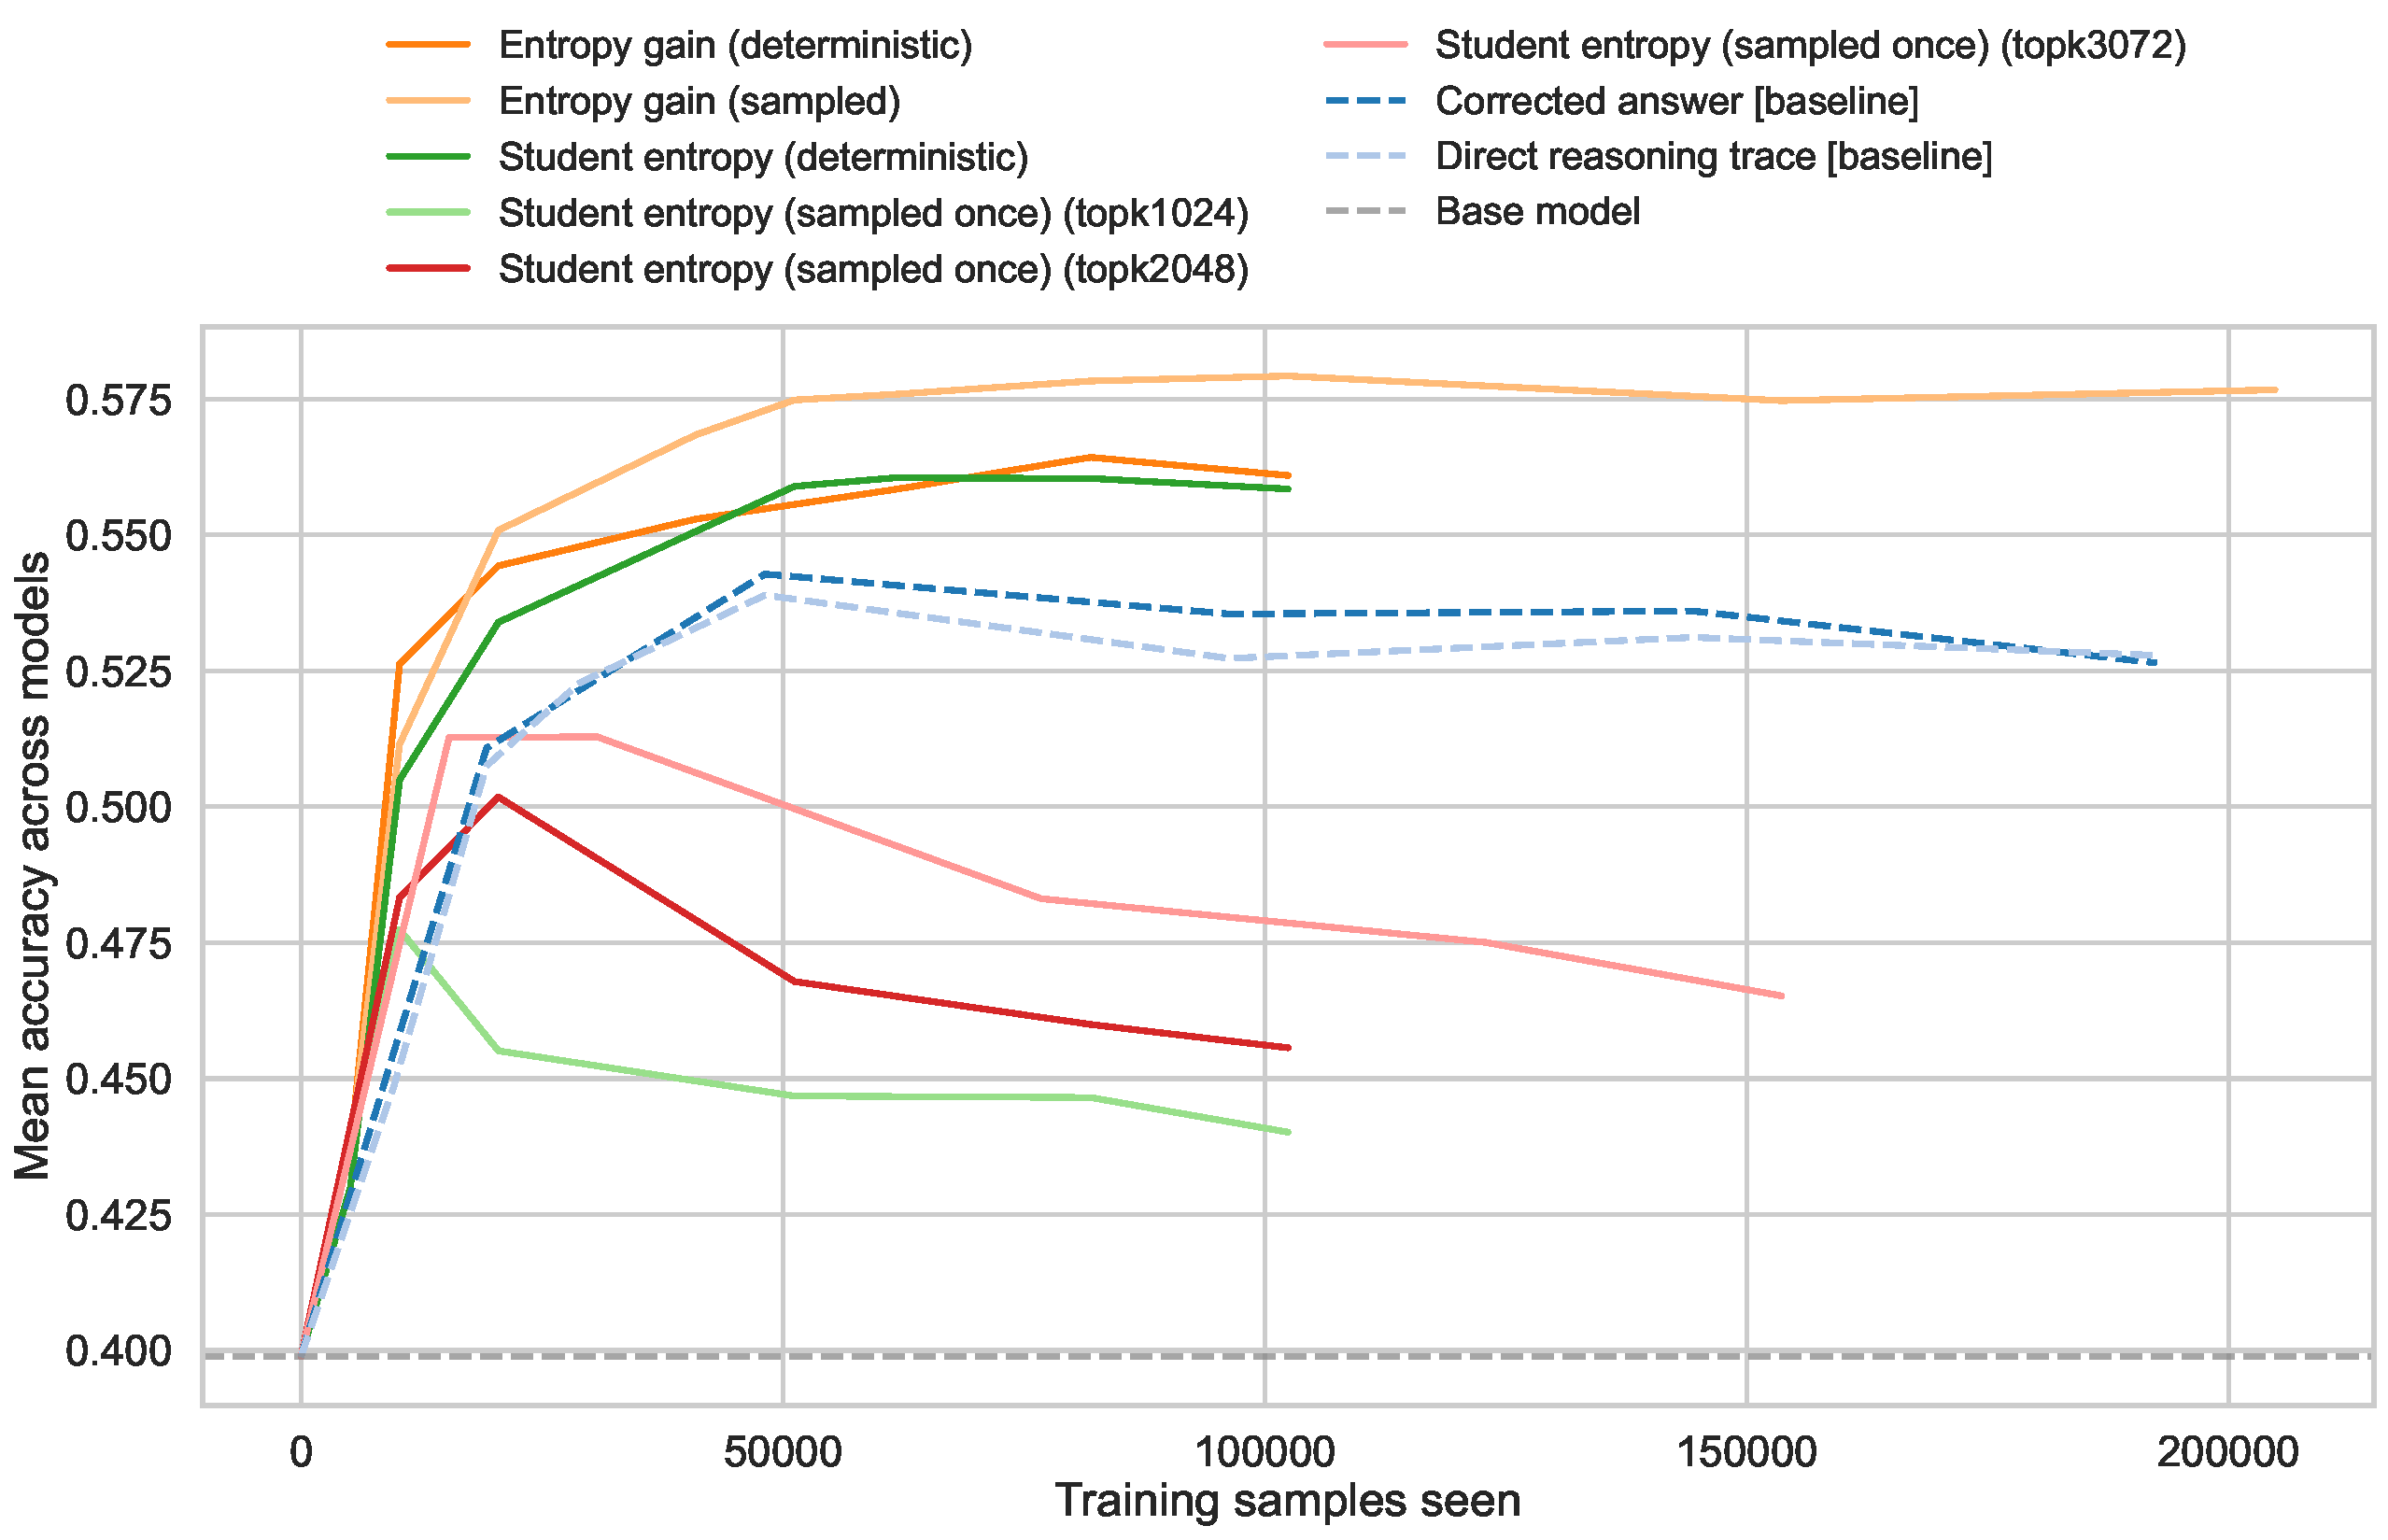
\includegraphics[width=1\linewidth]{img/all_models_reasoning_evals_cap2048.pdf}
    \caption{2048-token reasoning cap}
  \end{subfigure}
  \caption{Distillation pipeline results across three models (Qwen-3B, LLaMA-3B, and Phi4-mini) on MMLU-Pro}
  \label{fig:main_results_chraphs}
\end{figure*}

\begin{table*}[t]
  \centering
  \small
  \setlength{\tabcolsep}{4pt}
  \begin{tabular}{l *{4}{l}}
    \hline
    Method & \multicolumn{1}{c}{LLaMA-3B} & \multicolumn{1}{c}{Qwen-3B} & \multicolumn{1}{c}{Phi4-mini} & \multicolumn{1}{c}{Mean} \\
    \hline
    Direct reasoning trace & 46.09 / 45.55 & 51.45 / 50.37 & 57.27 / 62.43 & 51.61 / 52.78 \\
    Corrected answer & 47.80 / 47.26 & 50.87 / 49.42 & \underline{58.81} / 61.26 & 52.49 / 52.65 \\
    Student entropy (deterministic) & 49.83 / 50.08 & 53.62 / 53.03 & 58.35 / \underline{64.42} & \underline{53.93} / 55.85 \\
    Entropy gain (deterministic) & \underline{50.17} / \underline{50.37} & 51.04 / \underline{53.28} & 58.40 / \textbf{64.63} & 53.20 / \underline{56.10} \\
    Student entropy (sampled once, $k=1024$) & 41.35 / 40.11 & 39.44 / 39.07 & 50.17 / 52.87 & 43.65 / 44.01 \\
    Student entropy (sampled once, $k=2048$) & 42.19 / 41.06 & 43.18 / 43.02 & 53.20 / 52.62 & 46.19 / 45.57 \\
    Student entropy (sampled once, $k=3072$) & 42.02 / 42.81 & \textbf{56.77} / 40.86 & 56.77 / 55.90 & 51.86 / 46.52 \\
    Entropy gain (sampled) &
    \begin{tabular}[c]{@{}l@{}}\textbf{52.58} $\pm\,1.94$ /\\\textbf{52.08} $\pm\,2.28$
    \end{tabular} &
    \begin{tabular}[c]{@{}l@{}}\underline{56.64} $\pm\,3.79$ /\\\textbf{56.86} $\pm\,2.32$
    \end{tabular} &
    \begin{tabular}[c]{@{}l@{}}\textbf{62.22} $\pm\,2.42$ /\\64.07 $\pm\,4.52$
    \end{tabular} &
    \begin{tabular}[c]{@{}l@{}}\textbf{57.15} $\pm\,1.01$ /\\\textbf{57.67} $\pm\,1.19$
    \end{tabular} \\
    \hline
  \end{tabular}
  \caption{Distillation pipeline last epoch accuracy (\%) across three models (Qwen-3B, LLaMA-3B, and Phi4-mini) on MMLU-Pro, reported for 4096-token / 2,048-token thinking budget. Sampled entropy gain uses three seeds per model and includes $\pm$ 95\% confidence-interval. Other methods are deterministic.}
  \label{tab:distillation_main_results}
\end{table*}

\begin{figure}
  \centering
  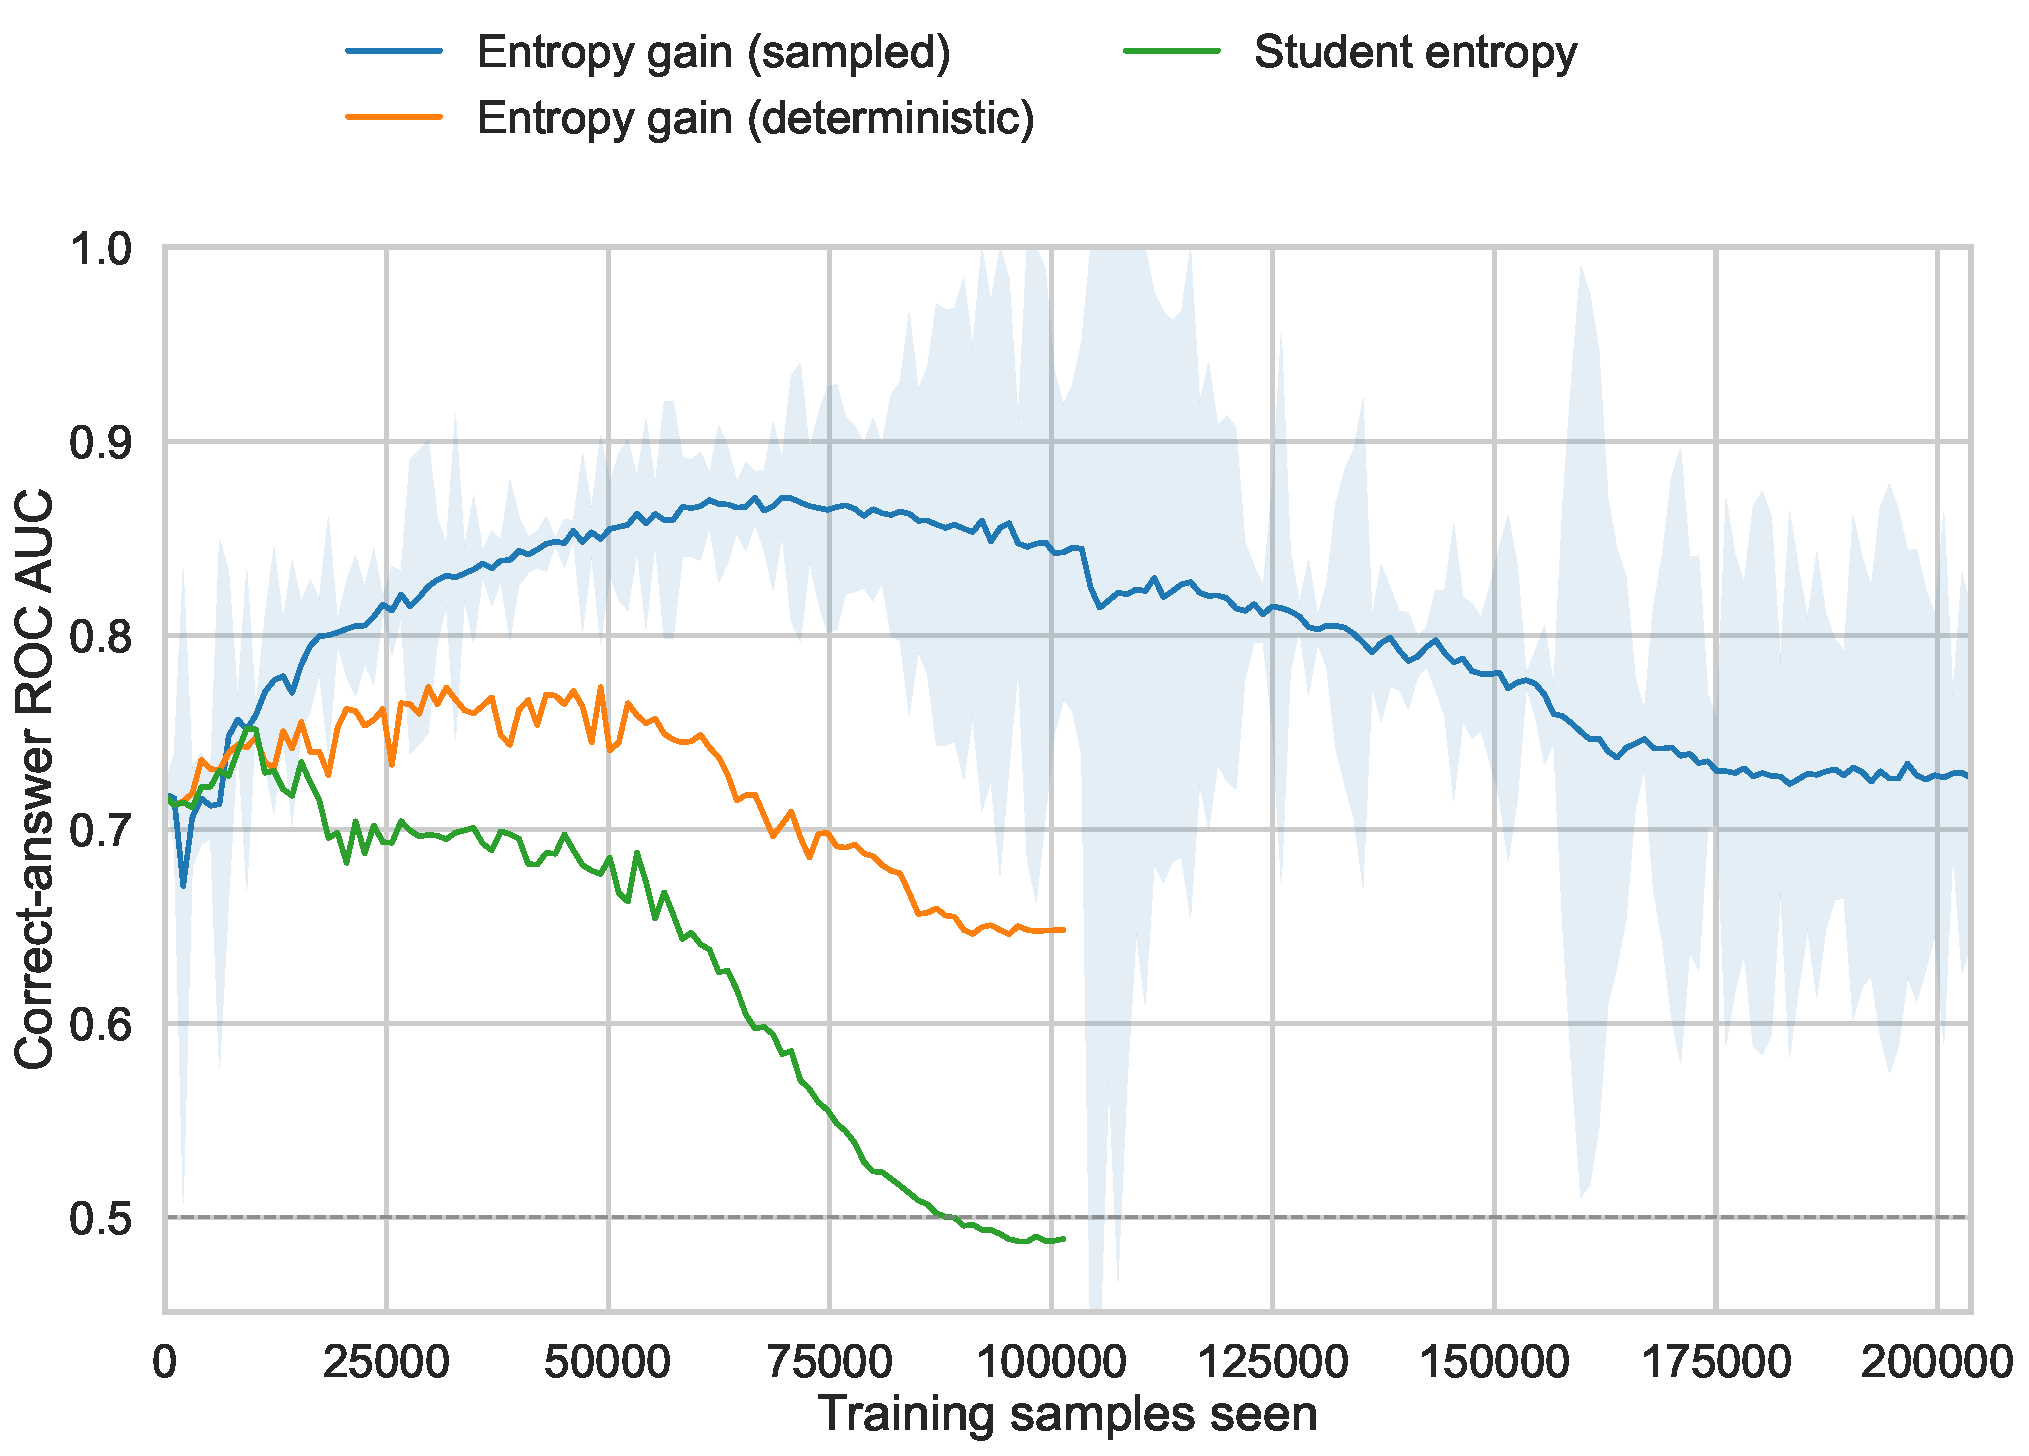
\includegraphics[width=1\linewidth]{img/student_entropy_roc_auc_all_models.pdf}
  \caption{Student calibration}
  \label{fig:student_calibration}
\end{figure}

\subsection{Synthetic Traces Generation}

\begin{figure*}
  \centering
  \begin{subfigure}[b]{0.31\linewidth}
    \centering
    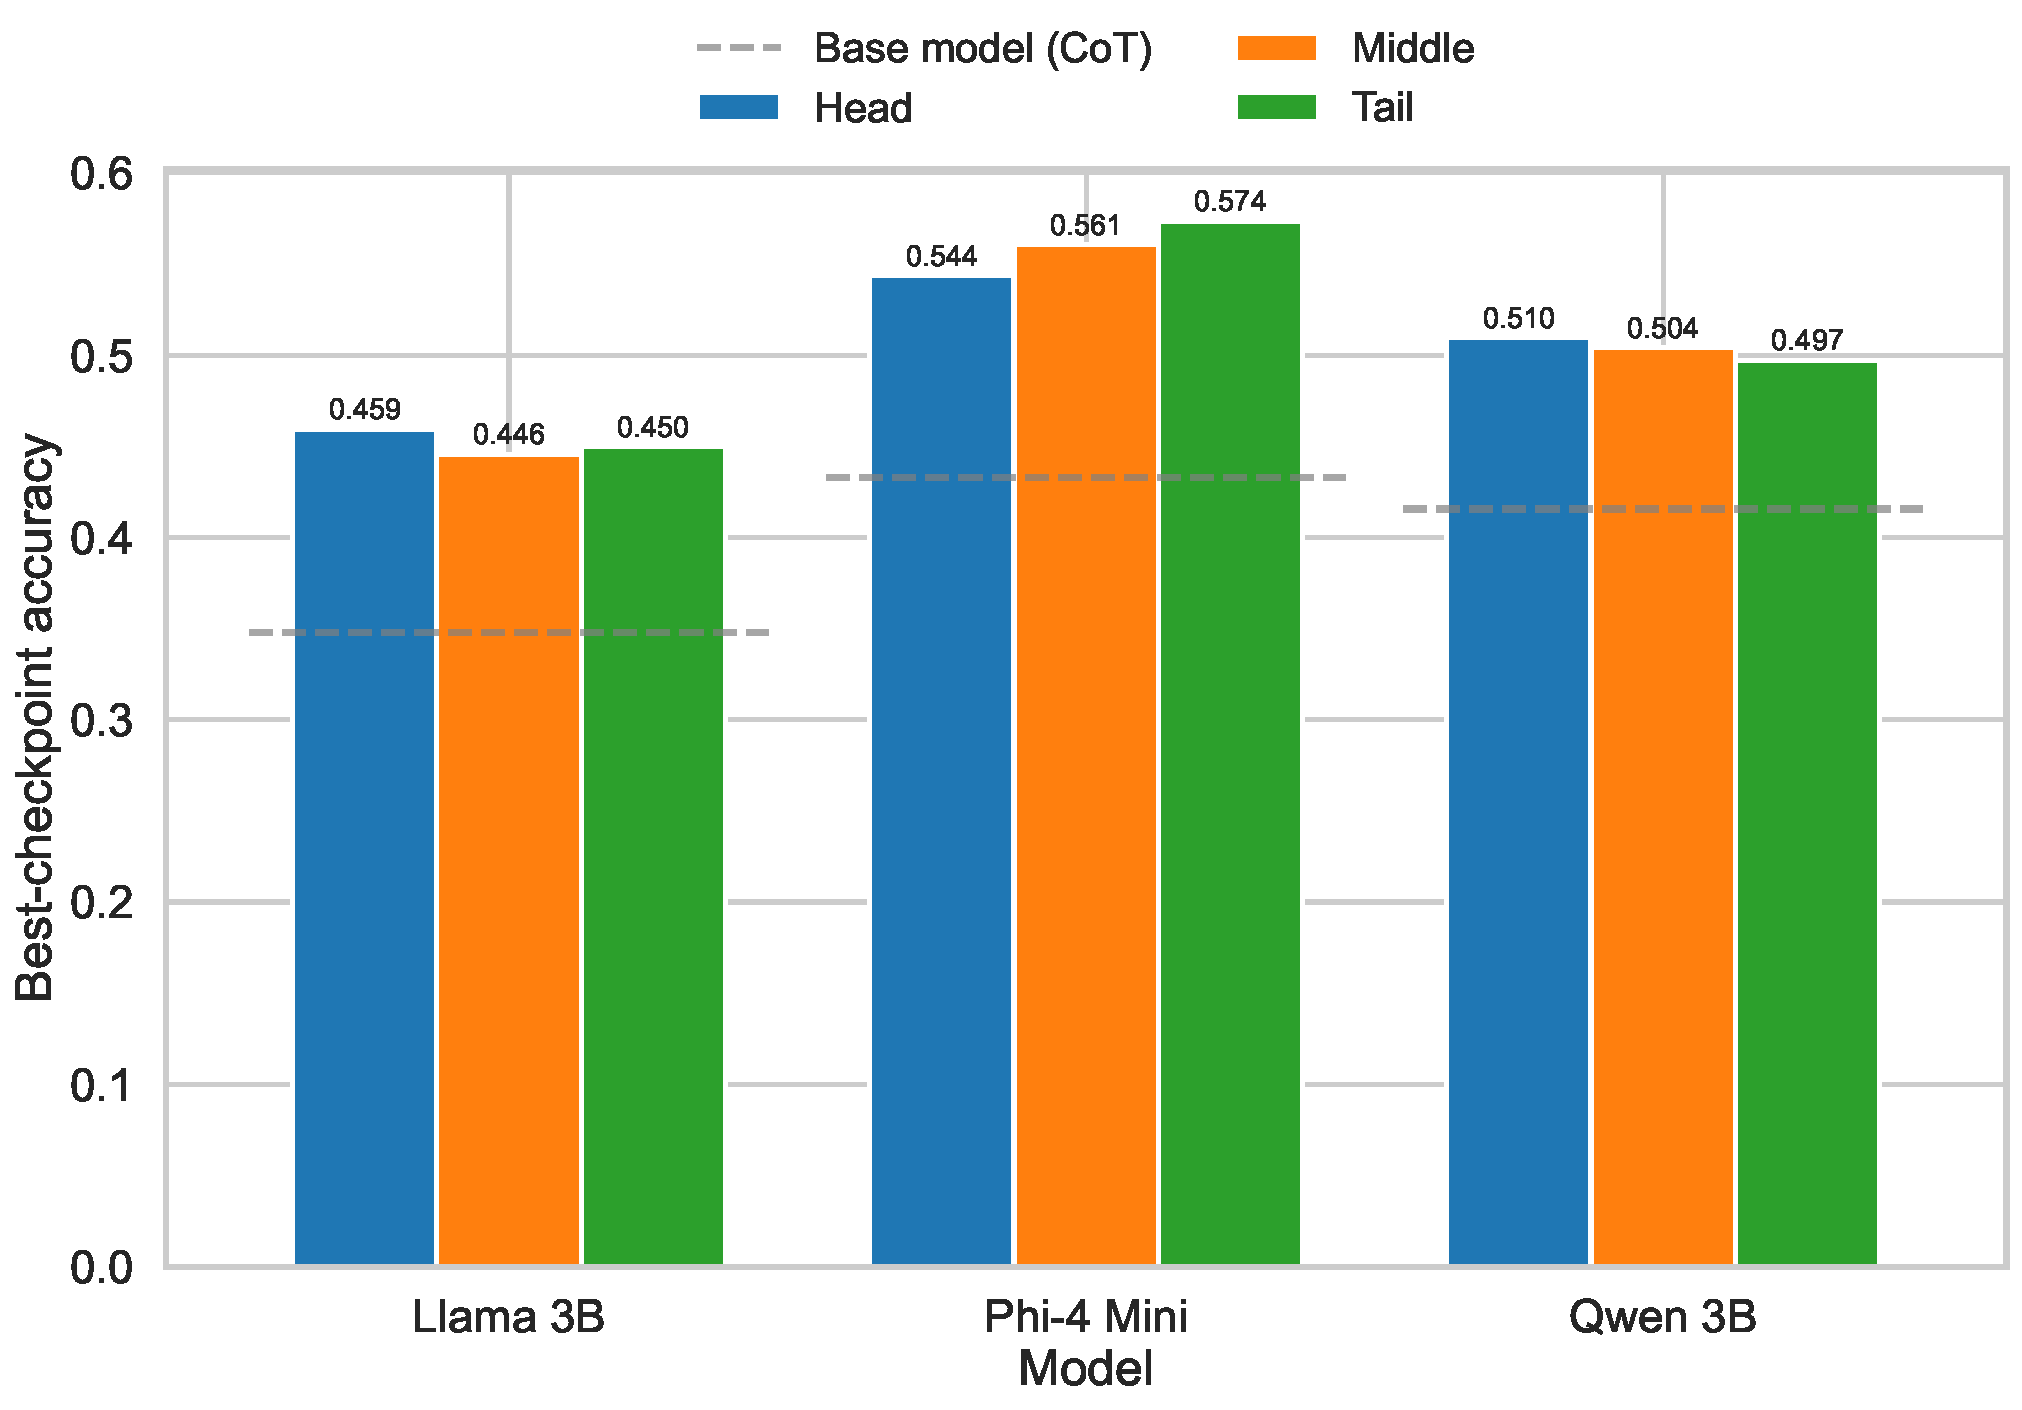
\includegraphics[width=1\linewidth]{img/performance_vs_truncation_mode_mode_best_acc_bars.pdf}
    \caption{by truncation}
  \end{subfigure}
  \hfill
  \begin{subfigure}[b]{0.30\linewidth}
    \centering
    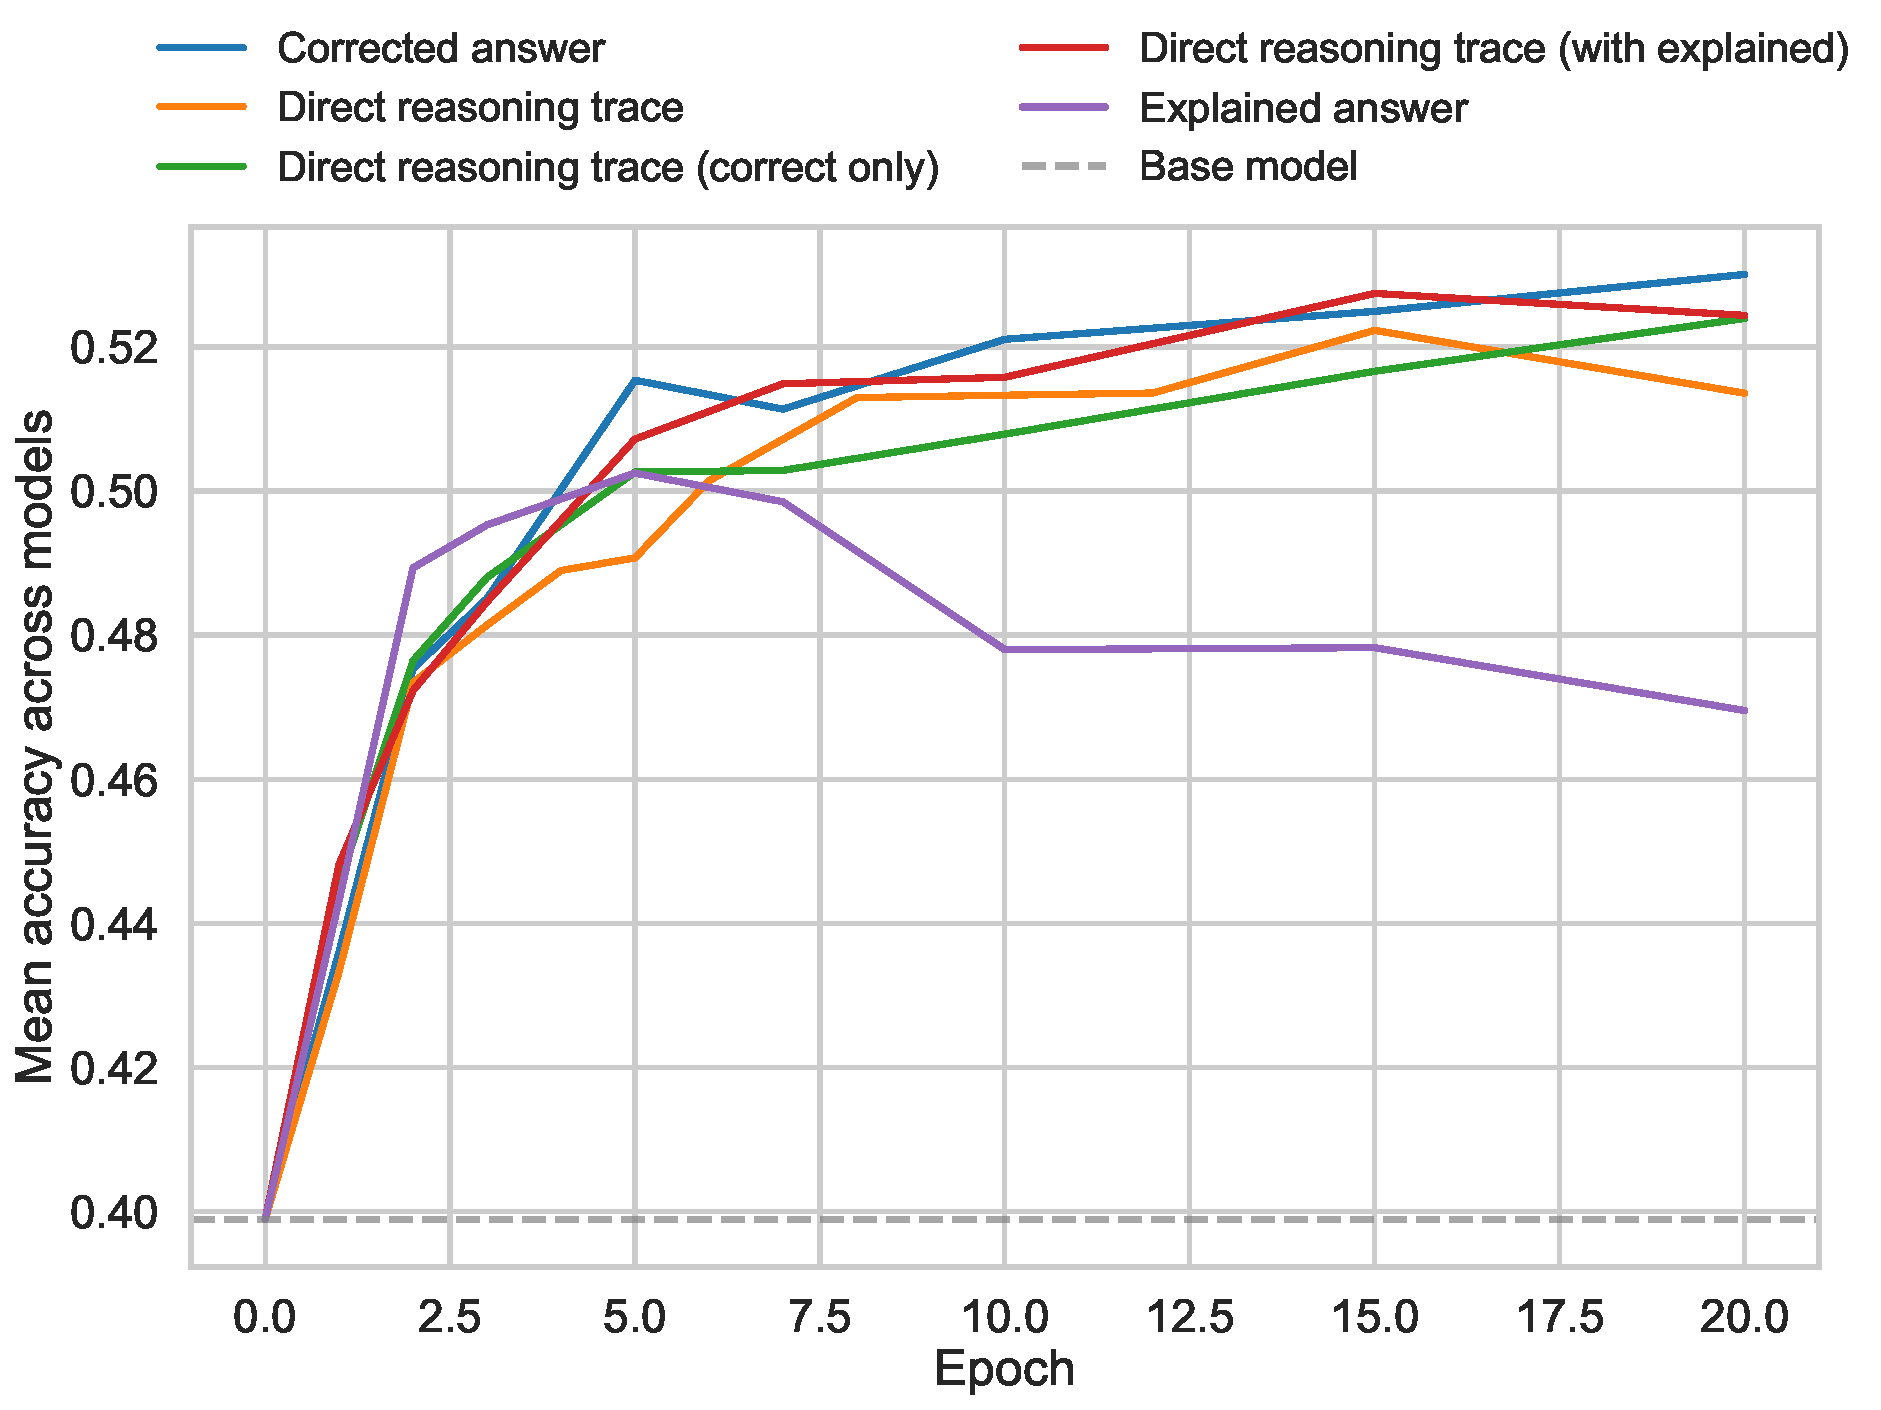
\includegraphics[width=1\linewidth]{img/distillation_on_synthetic_traces_all_models_head_truncated8192_reasoning_evals_mixed_caps.pdf}
    \caption{by type}
  \end{subfigure}
  \hfill
  \begin{subfigure}[b]{0.35\linewidth}
    \centering
    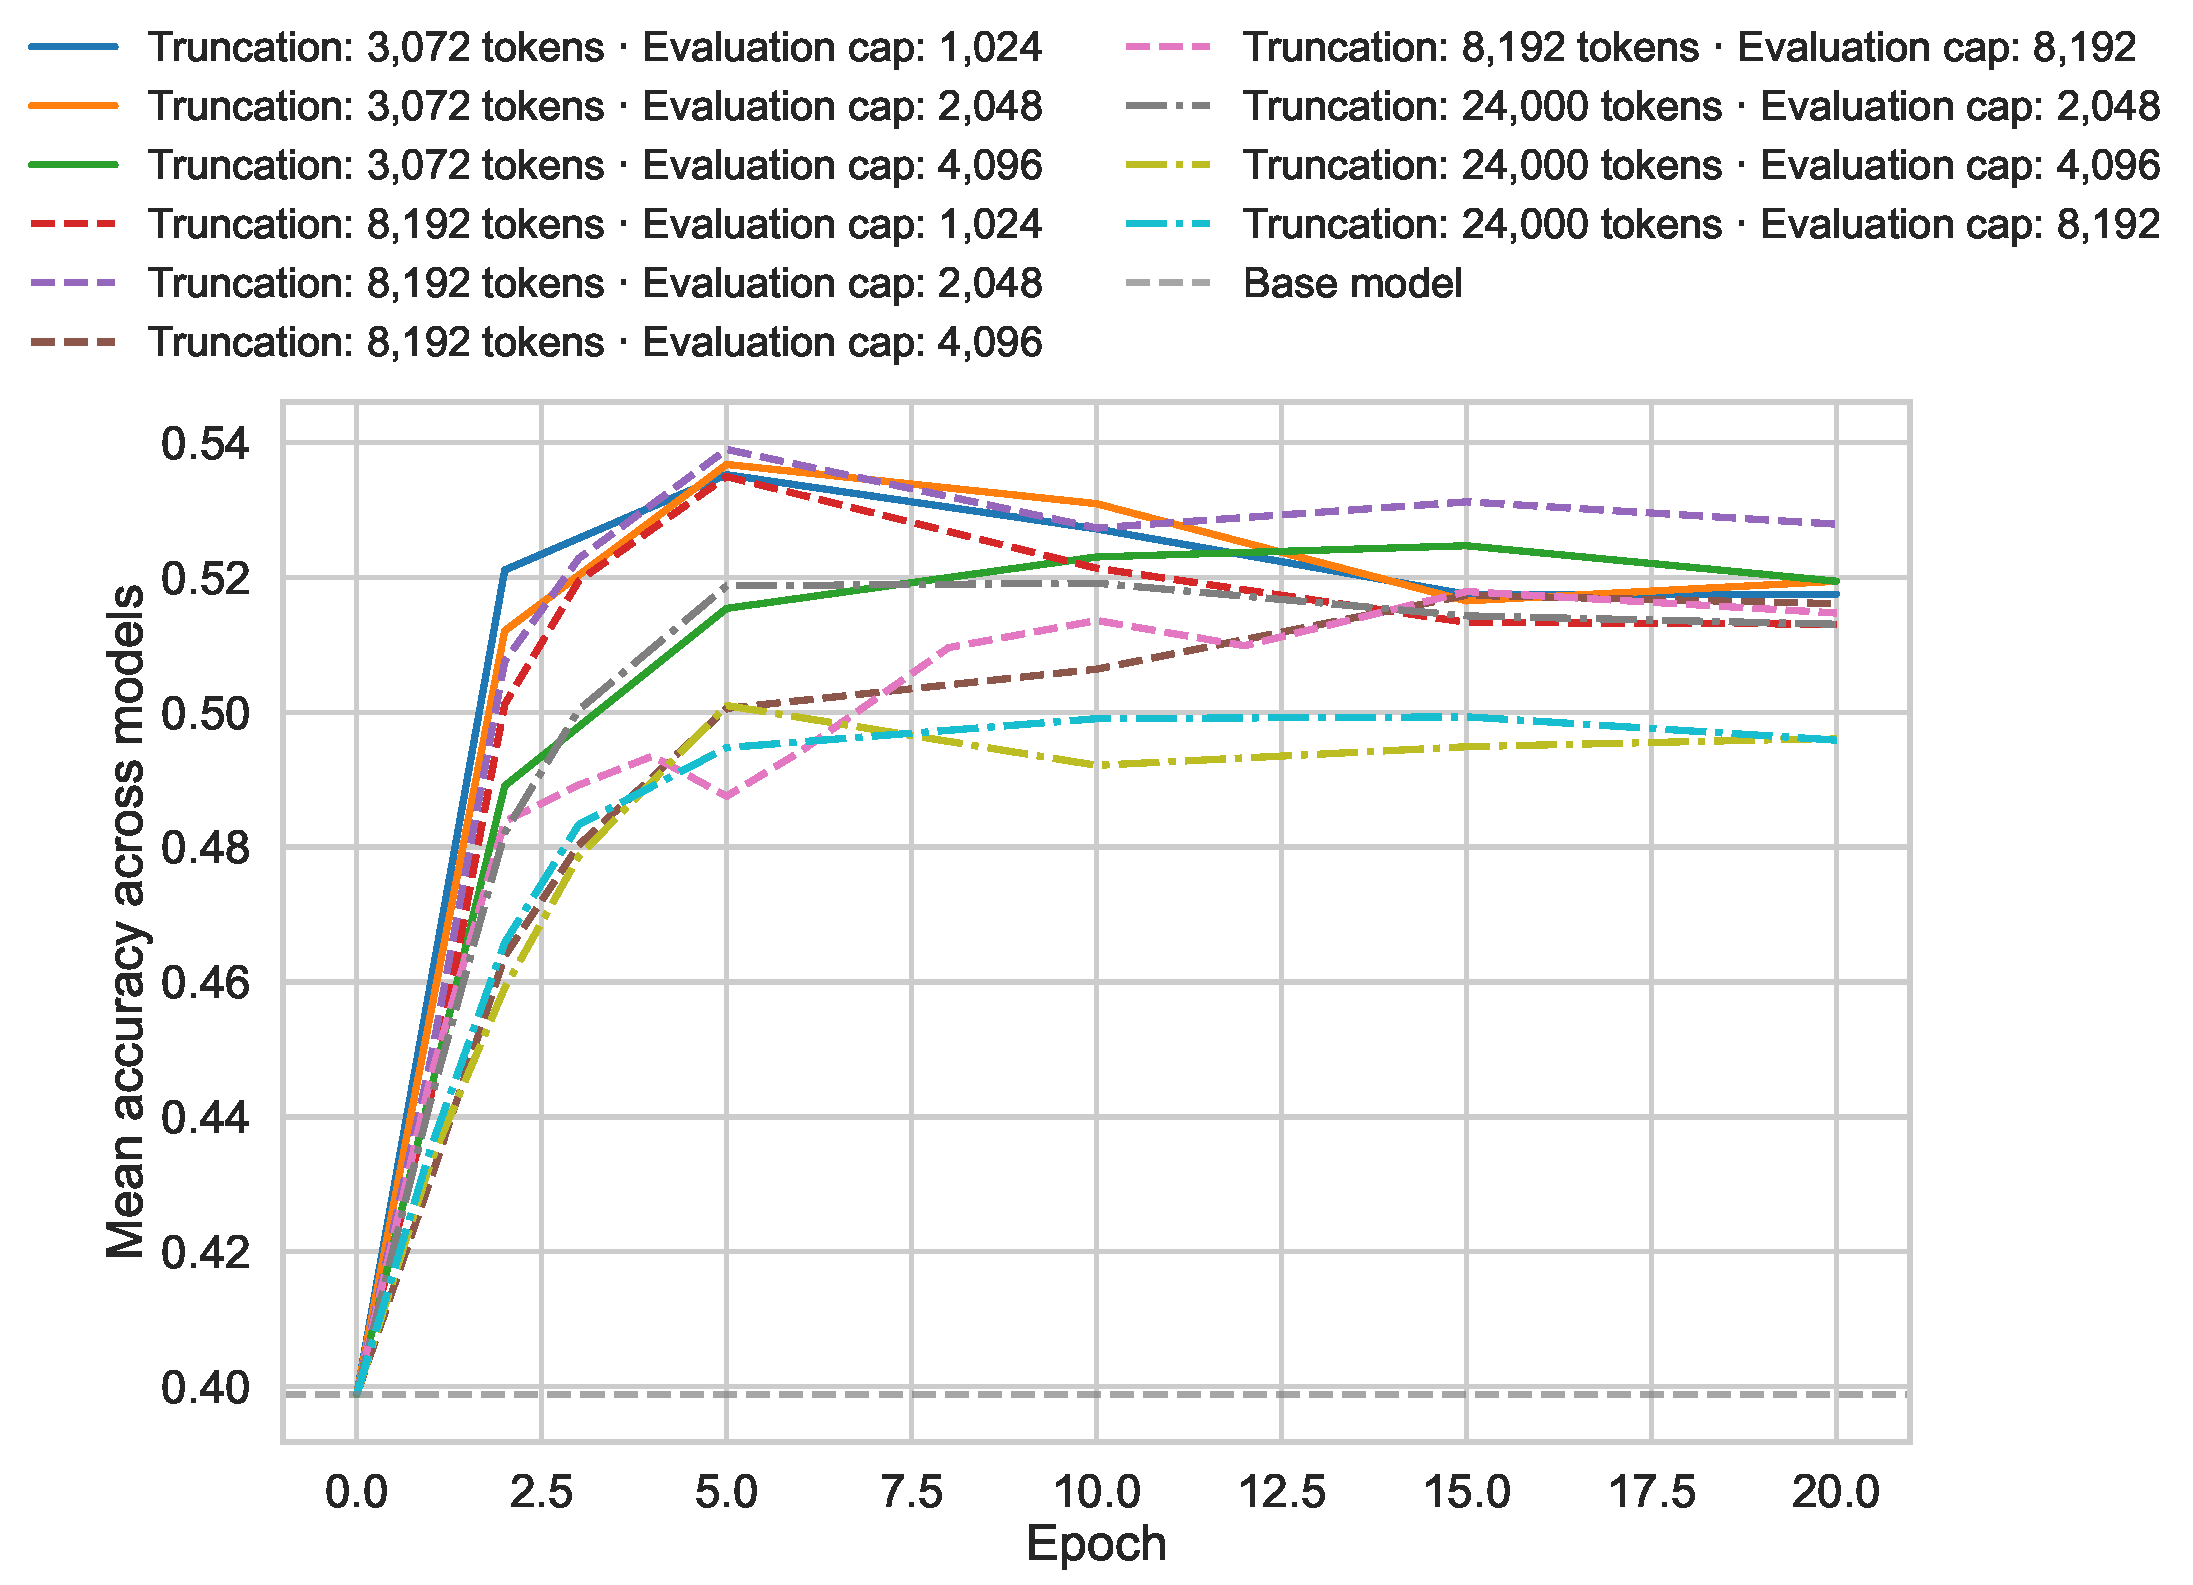
\includegraphics[width=1\linewidth]{img/distillation_on_synthetic_traces_all_models_head_truncated_by_model.pdf}
    \caption{by length}
  \end{subfigure}
  \caption{Comparison of synthetic traces}
  \label{fig:synth_comparison}
\end{figure*}

\subsection{Ablation Study}

\begin{figure*}
  \centering
  \begin{subfigure}[b]{0.48\linewidth}
    \centering
    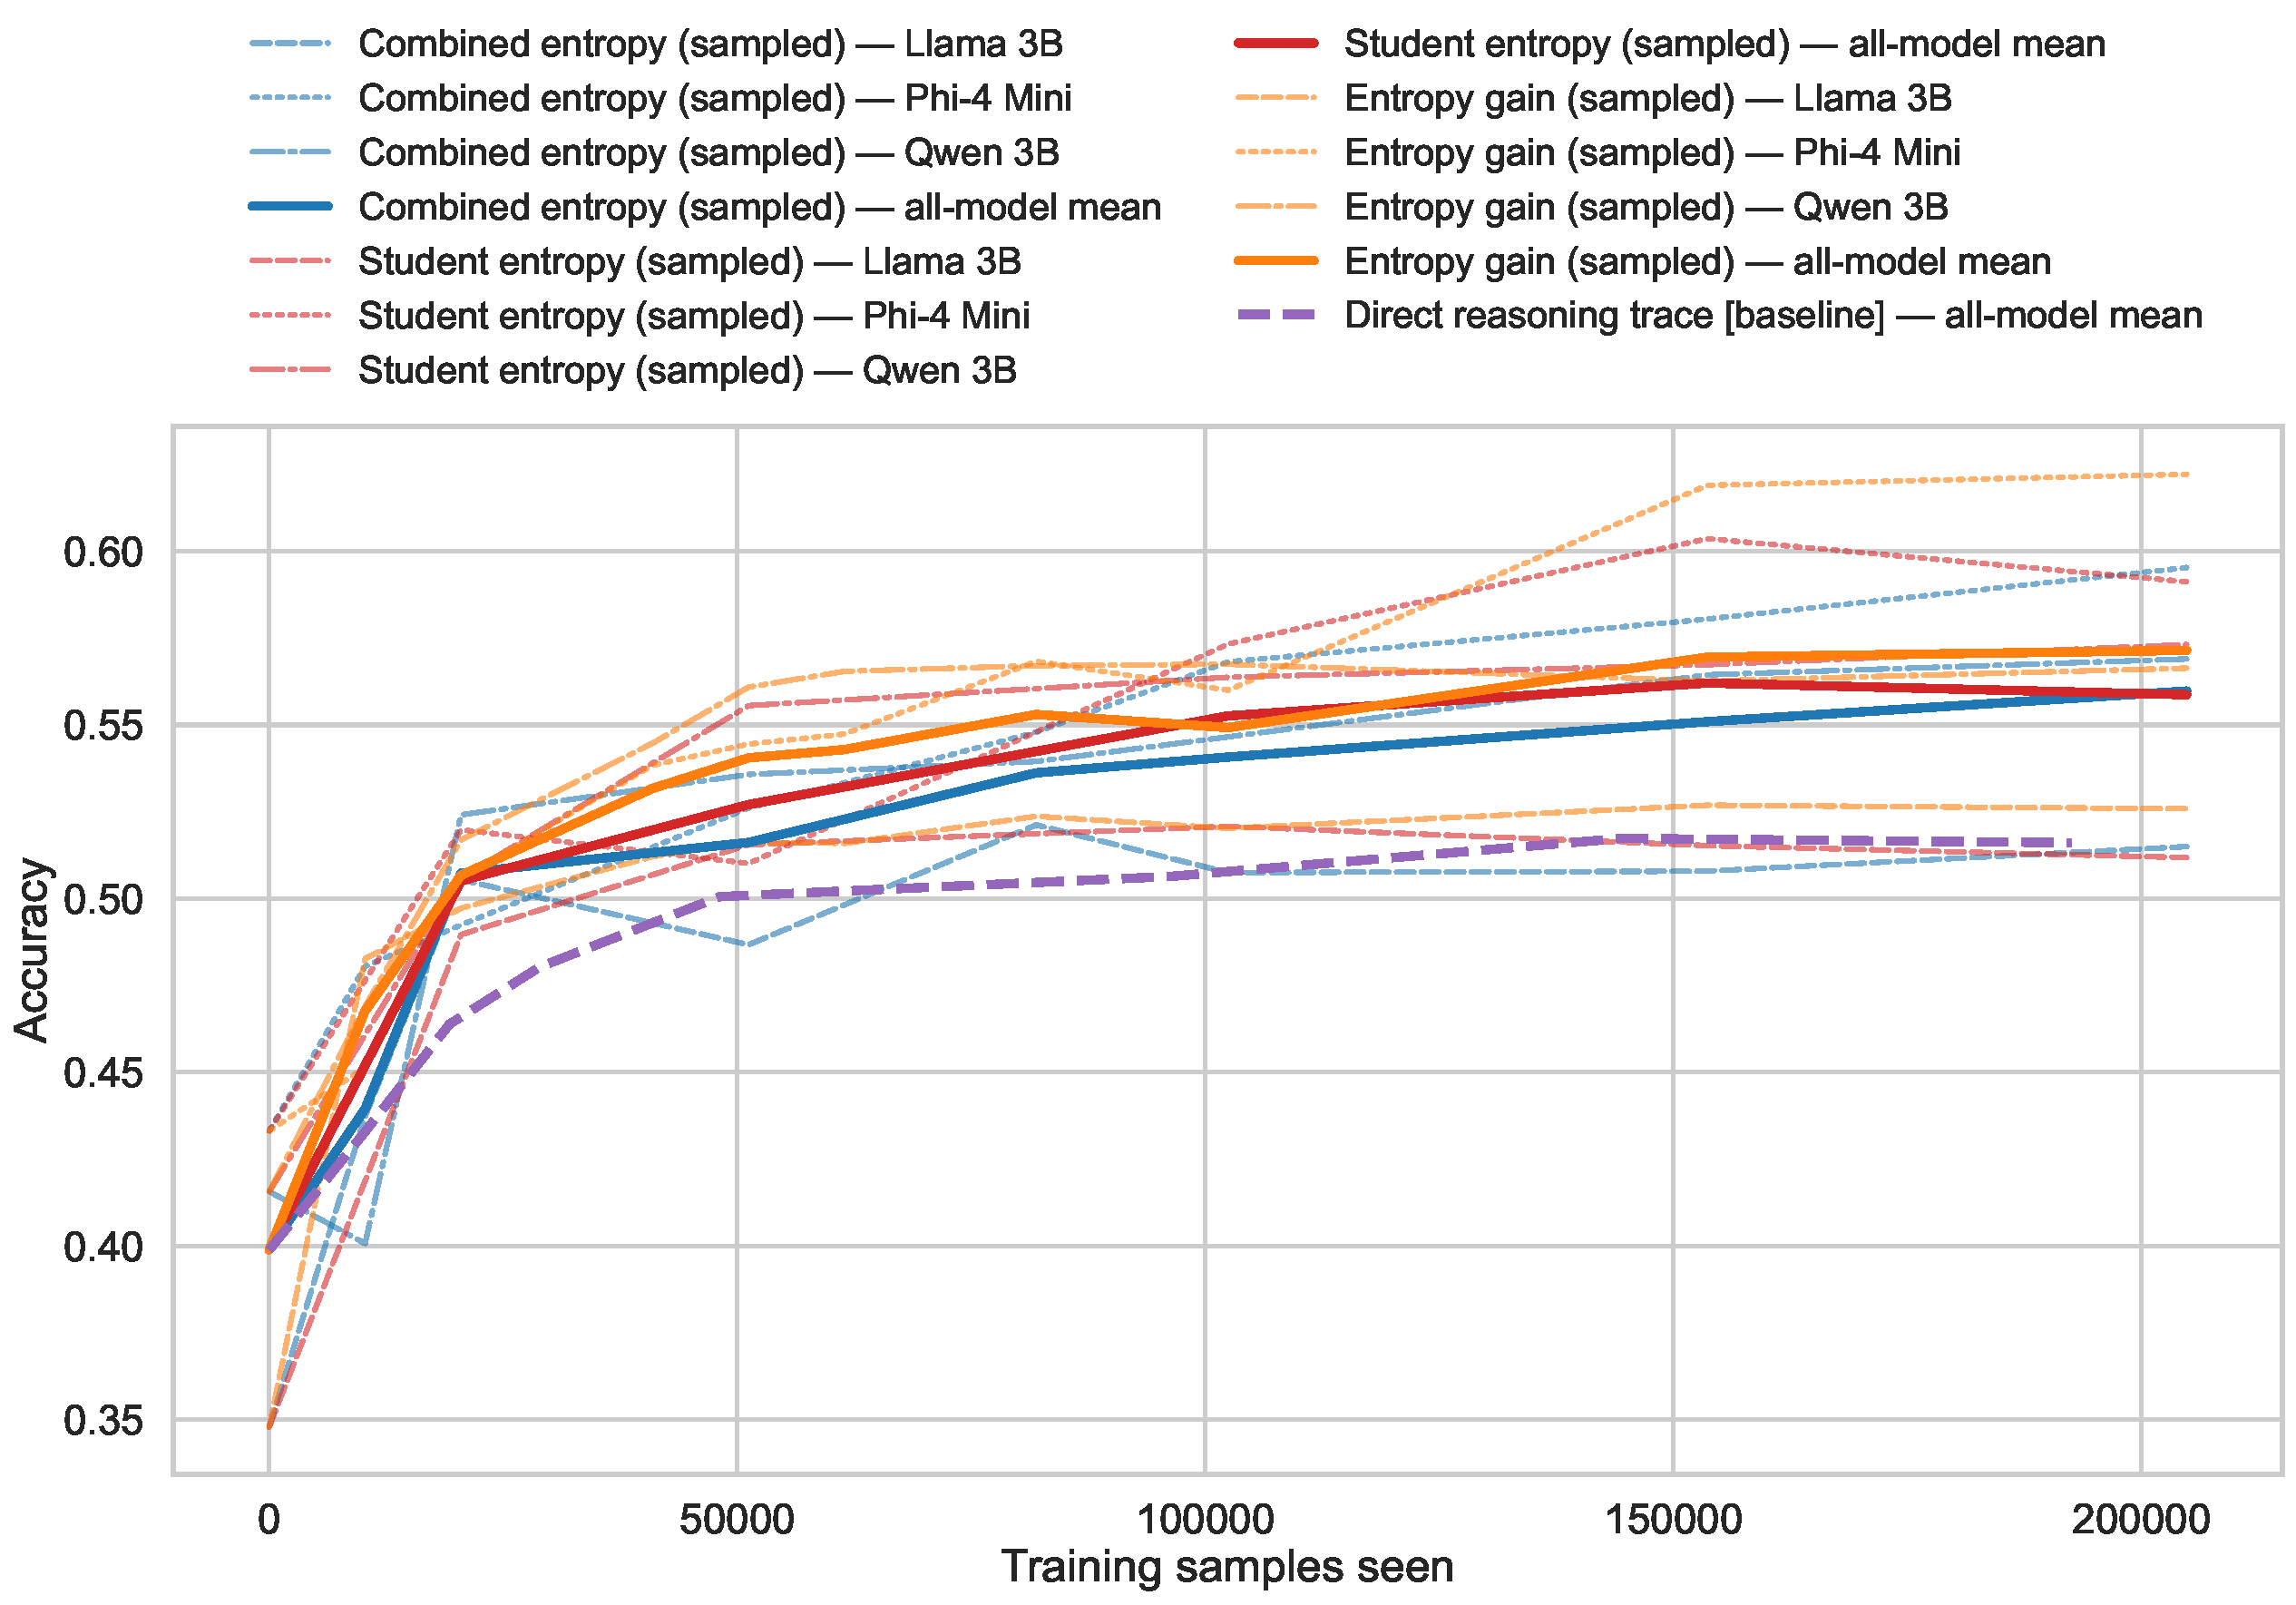
\includegraphics[width=1\linewidth]{img/proportional_samplers_reasoning_evals_cap4096.pdf}
    \caption{vs other entropy-based samplers}
  \end{subfigure}
  \hfill
  \begin{subfigure}[b]{0.48\linewidth}
    \centering
    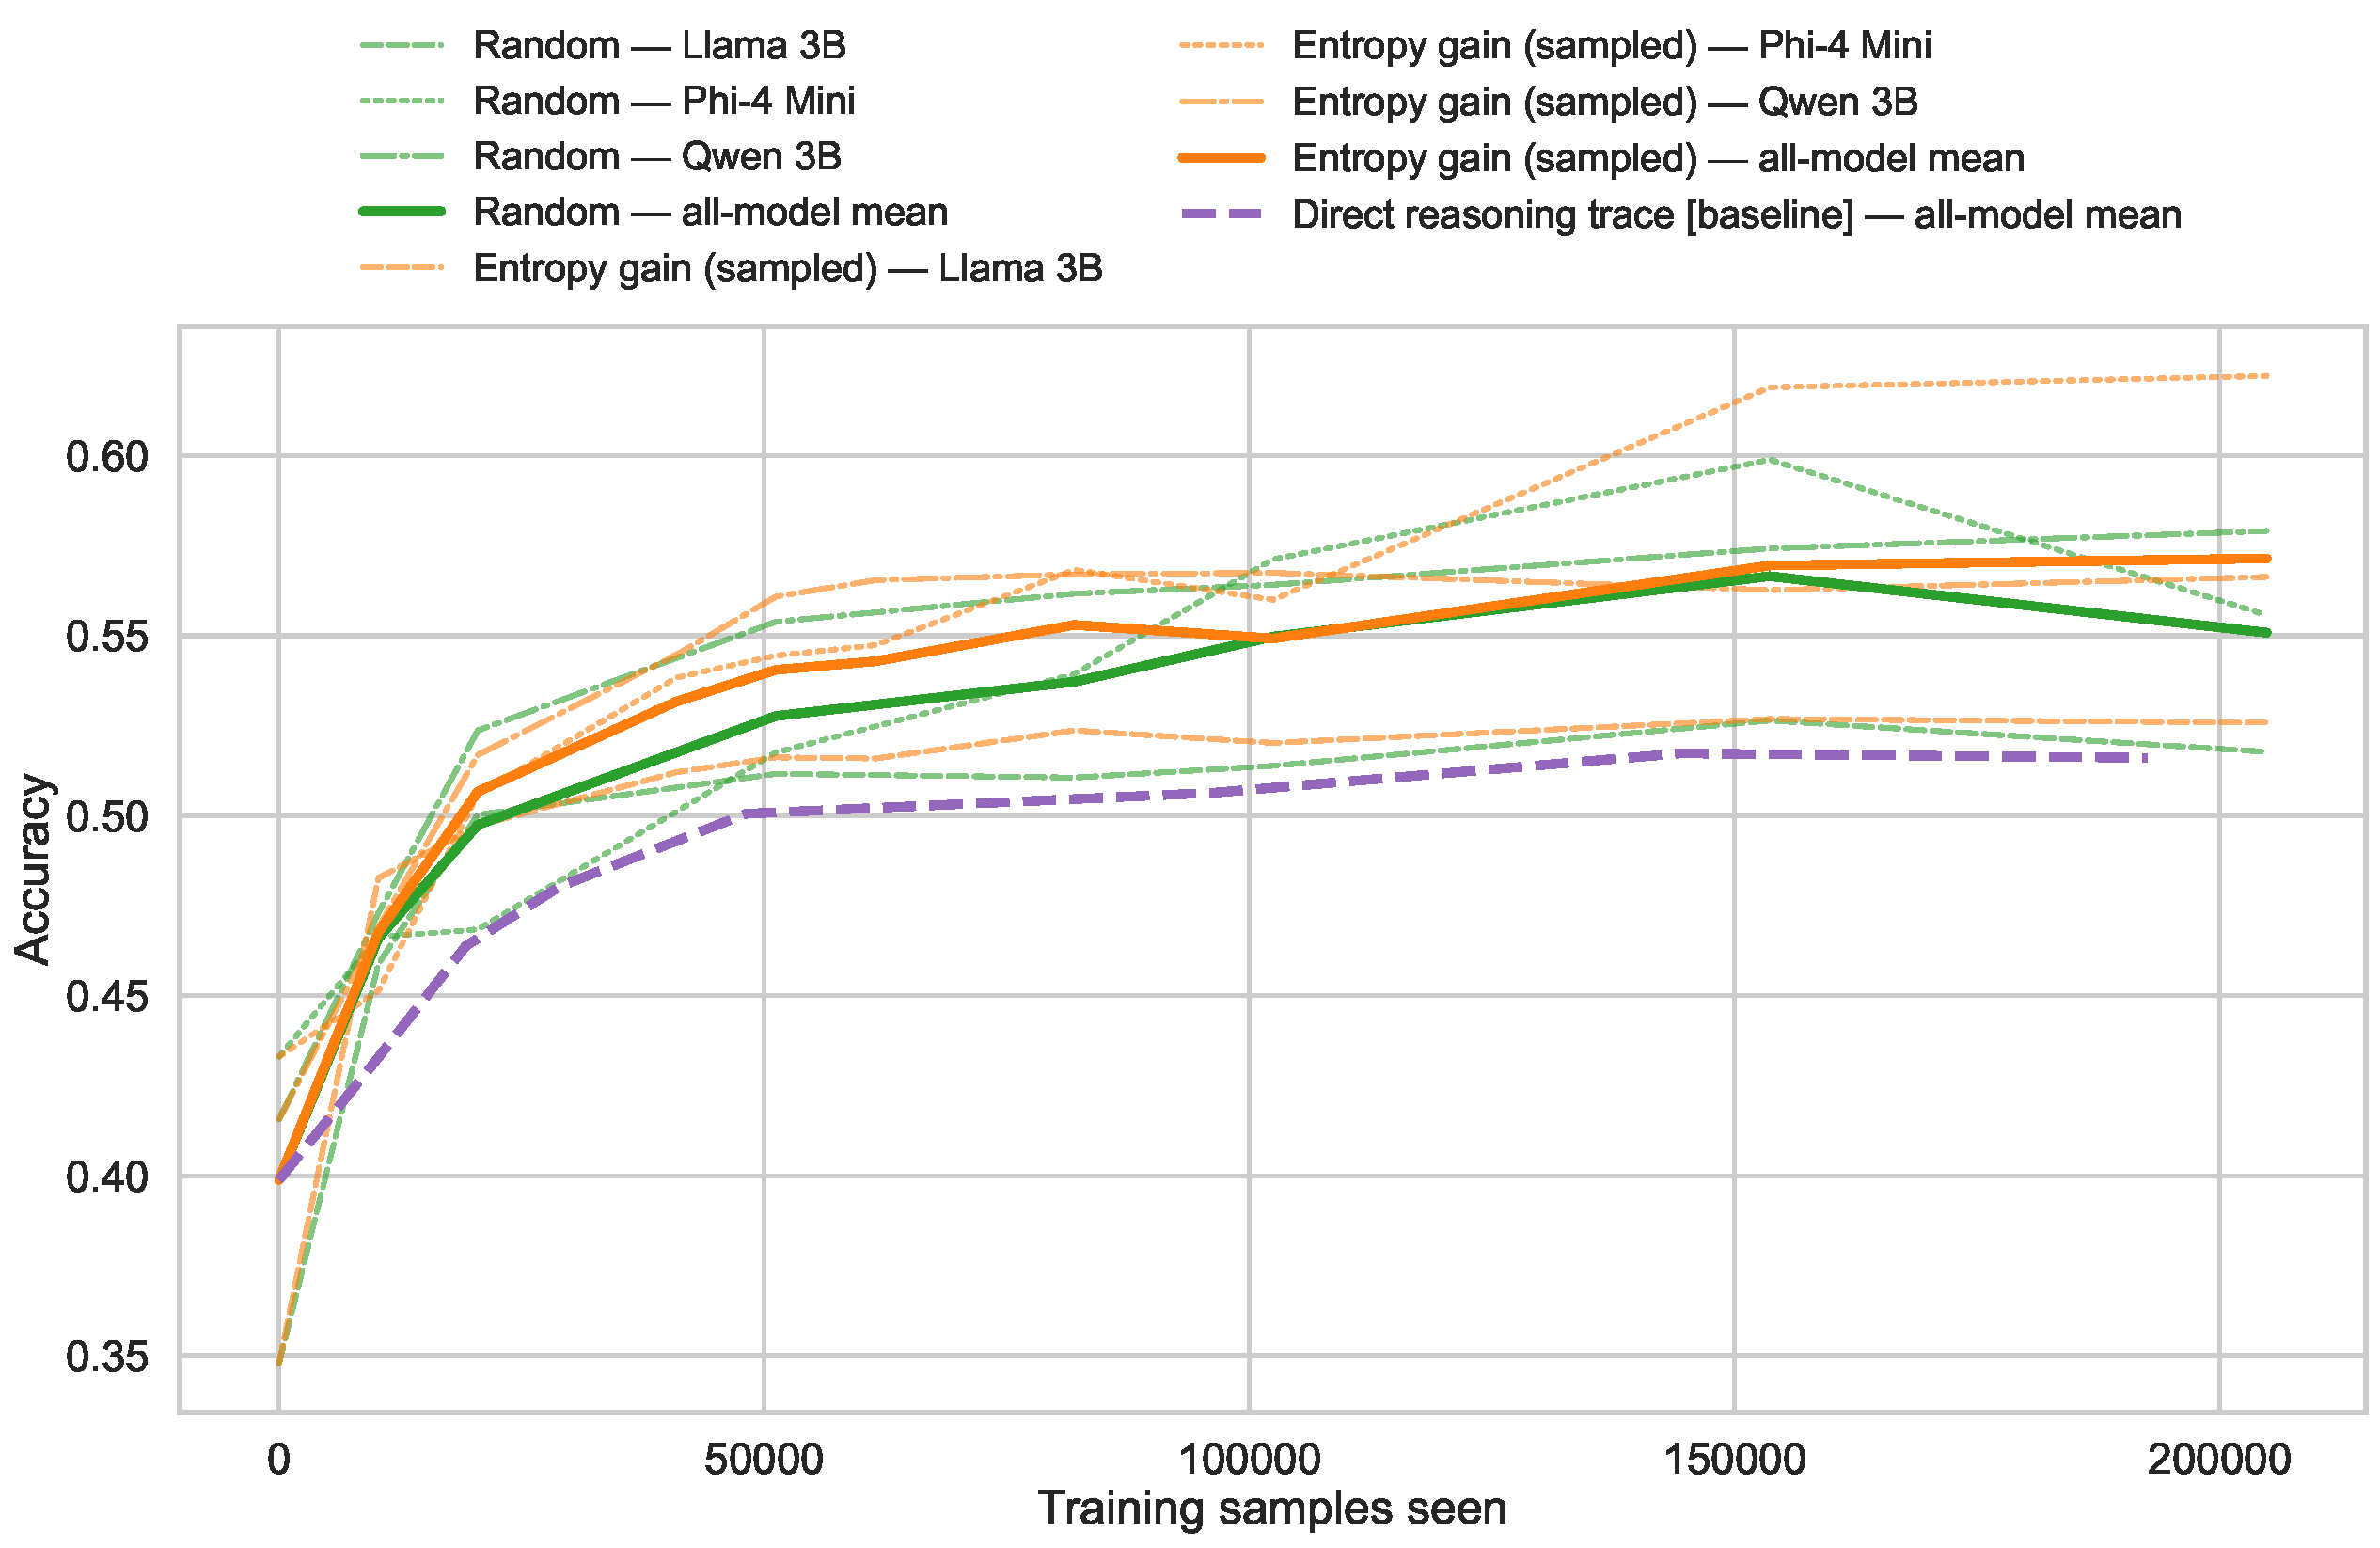
\includegraphics[width=1\linewidth]{img/random_vs_entropy_gain_proportional_reasoning_evals_cap4096.pdf}
    \caption{vs random sampler}
  \end{subfigure}
  \caption{Comparison of entropy gain sampler}
  \label{fig:entropy_gain_comparison}
\end{figure*}

\begin{table*}[t]
  \centering
  \small
  \setlength{\tabcolsep}{5pt}
  \begin{tabular}{l *{4}{r@{\,}l}}
    \hline
    Sampler & \multicolumn{2}{c}{LLaMA-3B} & \multicolumn{2}{c}{Qwen-3B} & \multicolumn{2}{c}{Phi4-mini} & \multicolumn{2}{c}{Mean} \\
    \hline
    Random & \underline{51.77} & $\pm\,2.76$ & \textbf{57.91} & $\pm\,1.40$ & 55.57 & $\pm\,2.54$ & 55.08 & $\pm\,0.80$ \\
    Student entropy & 51.18 & $\pm\,3.11$ & \underline{57.32} & $\pm\,1.52$ & 59.12 & $\pm\,5.22$ & 55.87 & $\pm\,1.40$ \\
    Combined entropy & 51.50 & & 56.90 & & \underline{59.53} & $\pm\,2.11$ & \underline{55.98} & \\
    Entropy gain & \textbf{52.58} & $\pm\,1.94$ & 56.64 & $\pm\,3.79$ & \textbf{62.22} & $\pm\,2.42$ & \textbf{57.15} & $\pm\,1.01$ \\
    \hline
  \end{tabular}
  \caption{Distillation pipeline last epoch accuracy for different sampling methods across three models (Qwen-3B, LLaMA-3B, and Phi4-mini) on MMLU-Pro, reported for 4096-token thinking budget. Each method is evaluated with 3 seeds per model and includes $\pm$ 95\% confidence-interval.}
  \label{tab:sampler_ablation}
\end{table*}

\section{Conclusion and discussion}

\section*{Limitations}

% Bibliography entries for the entire Anthology, followed by custom entries
%\bibliography{custom,anthology-overleaf-1,anthology-overleaf-2}

% Uncomment after adding a citation: an empty ACL bibliography causes a missing \item error.
%\bibliography{custom}

\appendix

\section{Example Appendix}
\label{sec:appendix}

This is an appendix.

\end{document}
